%\documentclass{article}
\documentclass{simulation}
%\documentclass[11pt,letterpaper]{report}
%\usepackage{psfig}

\usepackage{graphicx}
\graphicspath{ {} }	
\usepackage{bm}                                 
\usepackage{latexsym}
\usepackage{color}
\usepackage{amsmath}
\usepackage{verbatim}
\usepackage{amssymb}

\begin{document}

\section{Definition of classes}



\newpage \clearpage

\section{Field-theoretic treatment of interactions}

Our treatment of interactions uses a field-theoretic treatment of the densities to determine the interactions between polymer
segments.  Following work by de Pick, \emph{et al.}~\cite{pikeTheoreticallyInformedCoarse2009}, we define 

The simulation has a fixed volume with sides lengths $L_{x}$, $L_{y}$, and $L_{z}$.
These lengths are discretize into $M_{x}$, $M_{y}$, and $M_{z}$ bins of length
$\Delta_{x} = L_{x}/M_{x}$, 
$\Delta_{y} = L_{y}/M_{y}$, and 
$\Delta_{z} = L_{z}/M_{z}$.
The bins are defined by the three indices 
$i_{x}$,
$i_{y}$, and
$i_{z}$ that run from zero to 
$M_{x}-1$, 
$M_{y}-1$, and
$M_{z}-1$, respectively.


We consider the $n$th bead located at position $\vec{r}^{(n)}$.
We define a weight function $w_{I}(\vec{r}^{(n)})$ within the $I$th bin.  
The $I$th index is defined to be a superindex that combines 
$i_{x}$,
$i_{y}$, and
$i_{z}$ into a single unique index $I= i_{x} + M_{x} i_{y} + M_{x}M_{z} i_{z}$ that
runs from zero to $M_{x}M_{y}M_{z}-1$ (total of $M_{x}M_{y}M_{z}$ unique indices)
The total weight on the $I$th bin is given by the contributions from the three cartesian
directions, \emph{i.e.} 
$w_{I}(\vec{r}^{(n)}) = 
w_{i_{x}}^{(x)}(x^{(n)})
w_{i_{y}}^{(y)}(y^{(n)})
w_{i_{z}}^{(z)}(z^{(n)})$.
Figure~\ref{fig:weight} shows a schematic of the $x$-direction weight function (same method for $y$ and $z$).
This shows a linear interpolation weighting method, consistent with Ref.~\cite{pikeTheoreticallyInformedCoarse2009}.

\begin{figure}[b]
	\centering
	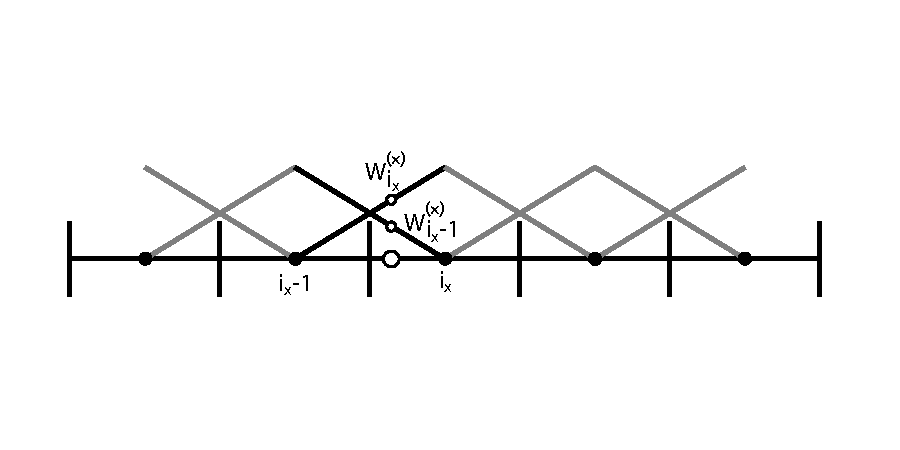
\includegraphics[width=0.6\textwidth]{figures/weight.pdf} 
    \caption{
    Schematic of the weight function $w_{i_{x}}^{(x)}$ that gives the weighting of the particle in the $i_{x}$ site in the
    $x$-direction based on a linear interpolation method~\cite{pikeTheoreticallyInformedCoarse2009}.
        }
        \label{fig:weight}
\end{figure}

The number of epigenetic proteins (\emph{e.g.} HP1) to the $n$th site is given by $N_{I}^{(\alpha)}$, where $\alpha$ determines
the type of epigenetic mark.
The $\alpha$-protein density within the $I$th bin is given by
\begin{equation}
\rho_{I}^{(\alpha)} = \frac{1}{v_{\mathrm{bin}}} \sum_{n=0}^{n_{b} - 1} w_{I}(\vec{r}^{(n)}) N_{I}^{(\alpha)}
\end{equation}
\noindent
where $v_{\mathrm{bin}} = \Delta_{x} \Delta_{y} \Delta_{z}$ is the volume of a bin.
The maximum number of epigenetic proteins bound $N_{\mathrm{max}}^{(\alpha)}$ gives an upper bound on the
number of proteins that can bind to a bead, accounting for coarse graining of a bead to represent multiple nucleosomes.
For discretization of one nucleosome per bead, the maximum $N_{\mathrm{max}}^{(\alpha)} = 2$ implies binding 
of a protein to the two histone tail proteins for the $\alpha$ epigenetic mark.
We define the number of $\alpha$ marks on the $I$th bead as $M_{I}^{(\alpha)}$, which can take values from zero
to $N_{\mathrm{max}}^{(\alpha)}$.

Protein binding to a marked tail results in energy $-\beta \epsilon_{m}$ [non-dimensionalized by $\beta = 1/(k_{B}T)$], and protein binding to an unmarked tail is associated with
energy $-\beta \epsilon_{u}$.  The chemical potential of the $\alpha$ protein is defined as $\beta \mu^{(\alpha)}$.
The binding of $N_{I}^{(\alpha)}$ proteins to a bead with $M_{I}^{(\alpha)}$ marks results in a free energy that 
accounts for all of the combinatoric ways of binding.

\section{Energetic contributions to the Monte Carlo simulation}

\subsection{Polymer chain model: shearable, stretchable wormlike chain}
We consider a polymer with $n_{b}$ number of beads.
We consider the shearable, stretchable wormlike chain potential, given by
\begin{equation}
\beta E_{\mathrm{elas}} = \sum_{n=0}^{n_{b}-2}
\left[
\frac{\epsilon_{\mathrm{b}}}{2 \Delta} \left| \vec{t}_{3}^{(n+1)} - \vec{t}_{3}^{(n)} - \eta \Delta \vec{r}_{\perp}^{(n)} \right|^{2} +
\frac{\epsilon_{\mathrm{\parallel}}}{2 \Delta} \left( \Delta \vec{r}^{(n)} \cdot \vec{t}_{3}^{(n)} - \Delta \gamma \right)^{2} +
\frac{\epsilon_{\mathrm{\perp}}}{2 \Delta} \left| \Delta \vec{r}_{\perp}^{(n)} \right|^{2}
\right],
\end{equation}
\noindent
where $\Delta \vec{r}^{(n)} = \vec{r}^{(n+1)} - \vec{r}^{(n)}$ is the bond vector,   
$\Delta \vec{r}_{\perp}^{(n)} = \Delta \vec{r}^{(n)} - (\Delta \vec{r}^{(n)} \cdot \vec{t}_{3}^{(n)}) \vec{t}_{3}^{(n)}$ is the
perpendicular component of the bond vector to the tangent vector. 



\bibliographystyle{unsrt}
\bibliography{chromo-derive}

\end{document}